\documentclass[a4paper, 11pt, oneside]{Dissertation}
\usepackage{times}
\usepackage{epsfig}
\usepackage{amsmath}
\usepackage{amssymb}
\usepackage{latexsym}
\usepackage{graphicx}
\usepackage{multirow}
\usepackage[english]{babel}
\usepackage{longtable}
\usepackage{algorithmicx}
\usepackage{algorithm}
\usepackage{algpseudocode}
\usepackage[numbers]{natbib}
\usepackage{enumitem}
\usepackage{xcolor}
\usepackage{tikz}
\usetikzlibrary{arrows.meta,positioning,shapes.geometric,fit,calc}
\usepackage{url}

\lstdefinestyle{DOS}
{
    backgroundcolor=\color{white},
    basicstyle=\scriptsize\color{black}\ttfamily
}
\lstset{basicstyle=\ttfamily\footnotesize,breaklines=true,frame=single,columns=fullflexible,
        keepspaces=true,showstringspaces=false}

\makeatletter
\def\BState{\State\hskip-\ALG@thistlm}
\makeatother

\usepackage{array}
\newcolumntype{L}[1]{>{\raggedright\let\newline\\\arraybackslash\hspace{0pt}}m{#1}}
\newcolumntype{C}[1]{>{\centering\let\newline\\\arraybackslash\hspace{0pt}}m{#1}}
\newcolumntype{R}[1]{>{\raggedleft\let\newline\\\arraybackslash\hspace{0pt}}m{#1}}

\graphicspath{{Figures/}{./}} % To include images in other directories

\long\def\symbolfootnote[#1]#2{\begingroup%
\def\thefootnote{\fnsymbol{footnote}}\footnote[#1]{#2}\endgroup}
\renewcommand{\baselinestretch}{1.2}
\onecolumn

% colours used by the architecture diagram (Chapter 3)
\definecolor{boxfill}{HTML}{f4f6fa}
% result numbers generated by benchmarks/plots.py (keeps text, tables and figures consistent)
% auto-generated by benchmarks/plots.py -- do not edit
\newcommand{\nUsers}{20}
\newcommand{\nQuestions}{330}
\newcommand{\llmName}{Qwen2.5-1.5B-Instruct}
\newcommand{\accNone}{18.2}
\newcommand{\accAnsNone}{0.0}
\newcommand{\halNone}{0.0}
\newcommand{\halAnsNone}{0.0}
\newcommand{\absNone}{100.0}
\newcommand{\tokNone}{117}
\newcommand{\latNone}{0.24}
\newcommand{\accNoneSH}{0.0}
\newcommand{\halNoneSH}{0.0}
\newcommand{\accNoneTC}{0.0}
\newcommand{\halNoneTC}{0.0}
\newcommand{\accNoneTB}{0.0}
\newcommand{\halNoneTB}{0.0}
\newcommand{\accNoneMH}{0.0}
\newcommand{\halNoneMH}{0.0}
\newcommand{\accNoneUN}{100.0}
\newcommand{\halNoneUN}{0.0}
\newcommand{\accFull}{57.3}
\newcommand{\accAnsFull}{61.1}
\newcommand{\halFull}{36.1}
\newcommand{\halAnsFull}{30.7}
\newcommand{\absFull}{40.0}
\newcommand{\tokFull}{4,209}
\newcommand{\latFull}{3.49}
\newcommand{\accFullSH}{62.4}
\newcommand{\halFullSH}{27.6}
\newcommand{\accFullTC}{80.0}
\newcommand{\halFullTC}{20.0}
\newcommand{\accFullTB}{13.3}
\newcommand{\halFullTB}{70.0}
\newcommand{\accFullMH}{77.5}
\newcommand{\halFullMH}{22.5}
\newcommand{\accFullUN}{40.0}
\newcommand{\halFullUN}{60.0}
\newcommand{\accWin}{26.4}
\newcommand{\accAnsWin}{11.1}
\newcommand{\halWin}{11.2}
\newcommand{\halAnsWin}{12.6}
\newcommand{\absWin}{95.0}
\newcommand{\tokWin}{664}
\newcommand{\latWin}{0.83}
\newcommand{\accWinSH}{10.0}
\newcommand{\halWinSH}{10.6}
\newcommand{\accWinTC}{30.0}
\newcommand{\halWinTC}{20.0}
\newcommand{\accWinTB}{0.0}
\newcommand{\halWinTB}{16.7}
\newcommand{\accWinMH}{10.0}
\newcommand{\halWinMH}{12.5}
\newcommand{\accWinUN}{95.0}
\newcommand{\halWinUN}{5.0}
\newcommand{\accRag}{73.6}
\newcommand{\accAnsRag}{73.3}
\newcommand{\halRag}{17.9}
\newcommand{\halAnsRag}{16.3}
\newcommand{\absRag}{75.0}
\newcommand{\tokRag}{266}
\newcommand{\latRag}{0.33}
\newcommand{\recRag}{90.4}
\newcommand{\mrrRag}{0.828}
\newcommand{\accRagSH}{80.6}
\newcommand{\halRagSH}{11.8}
\newcommand{\accRagTC}{86.7}
\newcommand{\halRagTC}{13.3}
\newcommand{\accRagTB}{50.0}
\newcommand{\halRagTB}{23.3}
\newcommand{\accRagMH}{50.0}
\newcommand{\halRagMH}{32.5}
\newcommand{\accRagUN}{75.0}
\newcommand{\halRagUN}{25.0}
\newcommand{\accMem}{78.2}
\newcommand{\accAnsMem}{80.0}
\newcommand{\halMem}{15.5}
\newcommand{\halAnsMem}{12.2}
\newcommand{\absMem}{70.0}
\newcommand{\tokMem}{267}
\newcommand{\latMem}{0.62}
\newcommand{\recMem}{96.3}
\newcommand{\mrrMem}{0.824}
\newcommand{\accMemSH}{81.2}
\newcommand{\halMemSH}{10.6}
\newcommand{\accMemTC}{90.0}
\newcommand{\halMemTC}{10.0}
\newcommand{\accMemTB}{63.3}
\newcommand{\halMemTB}{16.7}
\newcommand{\accMemMH}{80.0}
\newcommand{\halMemMH}{17.5}
\newcommand{\accMemUN}{70.0}
\newcommand{\halMemUN}{30.0}
\newcommand{\accMemGate}{80.6}
\newcommand{\accAnsMemGate}{79.3}
\newcommand{\halMemGate}{7.0}
\newcommand{\halAnsMemGate}{5.6}
\newcommand{\absMemGate}{86.7}
\newcommand{\tokMemGate}{267}
\newcommand{\latMemGate}{0.62}
\newcommand{\recMemGate}{96.3}
\newcommand{\mrrMemGate}{0.824}
\newcommand{\accMemGateSH}{80.6}
\newcommand{\halMemGateSH}{3.5}
\newcommand{\accMemGateTC}{90.0}
\newcommand{\halMemGateTC}{6.7}
\newcommand{\accMemGateTB}{60.0}
\newcommand{\halMemGateTB}{13.3}
\newcommand{\accMemGateMH}{80.0}
\newcommand{\halMemGateMH}{7.5}
\newcommand{\accMemGateUN}{86.7}
\newcommand{\halMemGateUN}{13.3}
\newcommand{\accRagGate}{74.8}
\newcommand{\accAnsRagGate}{72.2}
\newcommand{\halRagGate}{10.3}
\newcommand{\halAnsRagGate}{9.6}
\newcommand{\absRagGate}{86.7}
\newcommand{\tokRagGate}{266}
\newcommand{\latRagGate}{0.33}
\newcommand{\recRagGate}{90.4}
\newcommand{\mrrRagGate}{0.828}
\newcommand{\accRagGateSH}{79.4}
\newcommand{\halRagGateSH}{2.4}
\newcommand{\accRagGateTC}{86.7}
\newcommand{\halRagGateTC}{13.3}
\newcommand{\accRagGateTB}{46.7}
\newcommand{\halRagGateTB}{20.0}
\newcommand{\accRagGateMH}{50.0}
\newcommand{\halRagGateMH}{30.0}
\newcommand{\accRagGateUN}{86.7}
\newcommand{\halRagGateUN}{13.3}
\newcommand{\gatePMem}{0.93}
\newcommand{\gateRMem}{0.55}
\newcommand{\gateFMem}{0.69}
\newcommand{\gateFlaggedMem}{30}
\newcommand{\gateTPMem}{28}
\newcommand{\gateFPMem}{2}
\newcommand{\gateFNMem}{23}
\newcommand{\gatePosMem}{51}
\newcommand{\gatePRag}{0.89}
\newcommand{\gateRRag}{0.42}
\newcommand{\gateFRag}{0.57}
\newcommand{\gateFlaggedRag}{28}
\newcommand{\gateTPRag}{25}
\newcommand{\gateFPRag}{3}
\newcommand{\gateFNRag}{34}
\newcommand{\gatePosRag}{59}
\newcommand{\tokRatioFullMem}{16}
\newcommand{\latRatioFullMem}{6}
\newcommand{\rFiveVec}{90.4}
\newcommand{\rOneVec}{58.9}
\newcommand{\rThreeVec}{86.3}
\newcommand{\mrrLVec}{0.829}
\newcommand{\tempVec}{70.0}
\newcommand{\rFiveVecSH}{97.1}
\newcommand{\rFiveVecTC}{100.0}
\newcommand{\rFiveVecTB}{100.0}
\newcommand{\rFiveVecMH}{47.5}
\newcommand{\rFiveBm}{43.7}
\newcommand{\rOneBm}{24.1}
\newcommand{\rThreeBm}{41.1}
\newcommand{\mrrLBm}{0.439}
\newcommand{\tempBm}{26.7}
\newcommand{\rFiveBmSH}{44.1}
\newcommand{\rFiveBmTC}{30.0}
\newcommand{\rFiveBmTB}{43.3}
\newcommand{\rFiveBmMH}{52.5}
\newcommand{\rFiveHyb}{87.4}
\newcommand{\rOneHyb}{48.9}
\newcommand{\rThreeHyb}{79.6}
\newcommand{\mrrLHyb}{0.756}
\newcommand{\tempHyb}{65.0}
\newcommand{\rFiveHybSH}{91.2}
\newcommand{\rFiveHybTC}{93.3}
\newcommand{\rFiveHybTB}{93.3}
\newcommand{\rFiveHybMH}{62.5}
\newcommand{\rFiveQe}{89.6}
\newcommand{\rOneQe}{54.8}
\newcommand{\rThreeQe}{80.0}
\newcommand{\mrrLQe}{0.794}
\newcommand{\tempQe}{61.7}
\newcommand{\rFiveQeSH}{91.8}
\newcommand{\rFiveQeTC}{90.0}
\newcommand{\rFiveQeTB}{96.7}
\newcommand{\rFiveQeMH}{75.0}
\newcommand{\rFiveRr}{88.9}
\newcommand{\rOneRr}{54.1}
\newcommand{\rThreeRr}{84.1}
\newcommand{\mrrLRr}{0.801}
\newcommand{\tempRr}{60.0}
\newcommand{\rFiveRrSH}{91.8}
\newcommand{\rFiveRrTC}{93.3}
\newcommand{\rFiveRrTB}{96.7}
\newcommand{\rFiveRrMH}{67.5}
\newcommand{\rFiveGr}{90.7}
\newcommand{\rOneGr}{54.1}
\newcommand{\rThreeGr}{84.8}
\newcommand{\mrrLGr}{0.801}
\newcommand{\tempGr}{60.0}
\newcommand{\rFiveGrSH}{91.8}
\newcommand{\rFiveGrTC}{93.3}
\newcommand{\rFiveGrTB}{96.7}
\newcommand{\rFiveGrMH}{80.0}
\newcommand{\rFiveMem}{96.3}
\newcommand{\rOneMem}{56.7}
\newcommand{\rThreeMem}{88.9}
\newcommand{\mrrLMem}{0.827}
\newcommand{\tempMem}{80.0}
\newcommand{\rFiveMemSH}{98.8}
\newcommand{\rFiveMemTC}{90.0}
\newcommand{\rFiveMemTB}{93.3}
\newcommand{\rFiveMemMH}{92.5}
\newcommand{\pruneKeptThree}{55.5}
\newcommand{\pruneRecThree}{95.9}
\newcommand{\pruneKeptFortyFive}{16.9}
\newcommand{\pruneRecFortyFive}{92.6}
\newcommand{\pruneKeptFiftyFive}{9.6}
\newcommand{\pruneRecFiftyFive}{80.4}
\newcommand{\pruneRecZero}{96.3}
\newcommand{\niahMaxLen}{16k}
\newcommand{\niahNeedles}{8}
\newcommand{\niahCells}{200}
\newcommand{\niahFullAccFirst}{82.5}
\newcommand{\niahFullAccLast}{75.0}
\newcommand{\niahMemAccFirst}{90.0}
\newcommand{\niahMemAccLast}{72.5}
\newcommand{\niahFullAccMean}{80.0}
\newcommand{\niahMemAccMean}{83.5}
\newcommand{\niahFullAccMin}{75.0}
\newcommand{\niahMemAccMin}{72.5}
\newcommand{\niahMemRecallMean}{95.5}
\newcommand{\niahTokFullLast}{16,634}
\newcommand{\niahTokMemLast}{267}
\newcommand{\niahTokRatioLast}{62}
\newcommand{\niahLatFullLast}{81.6}
\newcommand{\niahLatMemLast}{0.70}
\newcommand{\niahLatFullFirst}{1.11}
\newcommand{\niahLatRatioLast}{117}
\newcommand{\niahMemMemories}{1118}


%% ----------------------------------------------------------------
\begin{document}
\sloppy
\pagenumbering{roman}

%%Cover Page
\thispagestyle{empty}
\begin{center}
{\Large \bf Context Window Analysis for Large Language Models:\\[4pt] Design and Evaluation of a Persistent Memory Layer}


\vspace*{1.5cm}
{\large Project report submitted in partial fulfillment\\}
{\large  of the requirements for the degree of \\}

\vspace*{1cm}
{\it {\large Bachelor of Technology} \\
{\large in\\}
{\large Communication and Computer Engineering \\}}

\vspace*{1cm}
{\large by}

\vspace*{1cm}
{\large Lakshya Jain - Roll No. 23UCS633\\}
{\large Monish Mathur - Roll No. 23UCS648\\}
{\large Nishit Luhadia - Roll No. 23UCC579\\}


\vspace*{5mm}
{\large Under Guidance of \\}
{\large Dr. Rahul Sharma \\}

\vspace*{1.0cm}
{
\psfig{figure= Figures/LNMIIT.png ,width=44mm}\\}

\vspace*{1.5cm}
{\large Department of Communication and Computer Engineering \\}
{\large The LNM Institute of Information Technology, Jaipur\\}

\vspace*{1.0cm}
{\large November 2026\\}
\end{center}

\clearpage


%% COPYRIGHT PAGE
\thispagestyle{empty}
\vfill
\begin{center}
\vspace*{\fill} \textcopyright \textbf{The LNM INSTITUTE OF INFORMATION TECHNOLOGY Jaipur-2026.}\\
\textbf{All rights reserved.}
\end{center}
\clearpage

%% CERTIFICATE PAGE
\newpage
\thispagestyle{empty}
\vspace*{1.5cm}

\begin{center}
{\Large The LNM Institute of Information Technology\\}
{\Large Jaipur, India\\}

\vspace*{3cm}

{\Large \bf CERTIFICATE\\}

\vspace*{1cm}
\end{center}

\noindent
This is to certify that the project entitled ``Context Window Analysis for Large Language Models: Design and Evaluation of a Persistent Memory Layer'', submitted by Lakshya Jain (Roll No: 23UCS633), Monish Mathur (Roll No: 23UCS648) and Nishit Luhadia (Roll No: 23UCC579) in partial fulfillment of the requirements for the degree of Bachelor of Technology (B.Tech), is a bonafide record of work carried out by them at the Department of Communication and Computer Engineering, The LNM Institute of Information Technology, Jaipur (Rajasthan), India, during the academic session 2026--2027, under my supervision and guidance. This work has not been submitted elsewhere for the award of any other degree. In my opinion, this report is of the standard required for the award of the degree of Bachelor of Technology (B.Tech).

\vspace*{3cm}

\begin{tabular}{cc}
\underline{\makebox[1.5in]{}} & \hspace*{4cm} \underline{\makebox[2.5in]{}} \\
Date & \hspace*{4cm} Adviser: Dr. Rahul Sharma
\end{tabular}


% ACKNOWLEDGEMENTS PAGE
\chapter*{Acknowledgments}
\label{ch:ack}

We would like to extend our sincere gratitude to our BTP mentor, Dr. Rahul Sharma, for his invaluable support, guidance, and consistent encouragement throughout both phases of this project. We also extend our thanks to the department faculty, staff, and our peers for their assistance and cooperation. Finally, we are deeply grateful to our friends and families for their unwavering motivation and support.


% Abstract
\chapter*{Abstract}
\label{ch:abstract}
Large Language Models (LLMs) are stateless: they answer only from the tokens in the current context
window, forget everything said in earlier sessions, and, as Phase 1 of this project showed, use long
contexts poorly and hallucinate even when retrieval is added. Phase 1 analysed these limitations and
proposed a persistent memory layer. This report describes Phase 2, in which the memory layer was built
and evaluated.

The implemented layer stores each conversation turn as a normalised note with an importance score, an
embedding in a FAISS index, BM25 tokens and extracted entities in a memory--entity graph. At query time
it combines dense and lexical retrieval with weighted reciprocal rank fusion, expands candidates through
the entity graph, re-ranks them with a cross-encoder, scores them with relevance-gated recency,
importance and coherence terms, resolves conflicting versions of a fact in favour of the newest, injects
the top five notes into a 512-token prompt, and verifies the generated answer with a grounding gate.

A long-term conversational benchmark with \nQuestions{} single-hop, temporal, multi-hop and unanswerable
questions over \nUsers{} multi-session histories was built, and five strategies were compared with the
same local model (\llmName): no memory, full conversation history, sliding window, the Phase-1
vector-RAG design and the proposed layer. The memory layer with its gate reached \accMemGate\% accuracy
and a \halMemGate\% hallucination rate, against \accFull\% and \halFull\% for the full history and
\accRag\% and \halRag\% for vector RAG, while using \tokRatioFullMem{} times fewer prompt tokens than the
full history. An ablation attributes the gains to the entity graph (multi-hop retrieval recall
\rFiveVecMH\% $\rightarrow$ \rFiveMemMH\%), the conflict-aware update rule and memory scoring; importance
pruning keeps full recall with half of the turns; and the grounding gate detects hallucinations with
precision \gatePMem{} and F1 \gateFMem{} compared with 0.25 and 0.39 for the detectors studied in Phase 1.
A needle-in-a-haystack experiment on histories up to \niahMaxLen{} tokens confirms that the layer's cost
stays constant while full-context cost grows linearly. The results support the project's thesis that a
selective, verified memory is a better basis for long-running LLM applications than a larger context
window.


\pagestyle{fancy}
%--------------------------------------------------------
\tableofcontents
\listoffigures
\listoftables
\newpage

%% ----------------------------------------------------------------
\mainmatter

\chapter{Introduction}
\label{ch:intro}

\section{The Area of Work}
Large Language Models (LLMs) are now used in chatbots, coding assistants, customer support systems and
personal assistants that people talk to over days, weeks and months. The underlying Transformer
architecture, however, is stateless: every request is answered only from the tokens that fit in the current
context window. Everything that was said in an earlier session is forgotten unless it is sent again.

This project lies at the intersection of Large Language Models, text embeddings, vector databases,
information retrieval and knowledge graphs. The first phase of the project (April 2026) analysed the
limitations of the context window and of Retrieval-Augmented Generation (RAG), and \emph{proposed} a
persistent memory layer. This second phase \emph{builds} that memory layer, benchmarks it against the
alternatives, and reports what works and what does not.

\section{Problem Addressed}
In Phase 1 we established, using the RAGTruth dataset and Needle-in-a-Haystack (NIAH) experiments, two
limitations of current systems:
\begin{itemize}[nosep]
  \item LLMs do not use long contexts effectively. Accuracy drops as the context grows and depends on
        \emph{where} the relevant information sits (``lost in the middle'').
  \item Retrieval alone does not remove hallucination. Hallucination detectors on RAGTruth reached high
        recall (0.88--0.95) but very low precision (0.25--0.26), i.e.\ an F1 of only about 0.4.
\end{itemize}
Phase 1 therefore proposed a memory layer that stores conversation turns as embeddings in a vector
database and injects only the most relevant memories into the prompt. Its future-work section listed the
concrete components that were still missing: hybrid vector + BM25 search, a multi-stage retrieval pipeline
with re-ranking, query expansion, memory scoring with ageing, a graph-based memory representation, an
end-to-end pipeline, and a comparative evaluation against baseline LLMs and RAG.

The problem addressed in this phase is to turn that proposal into a working, measurable system and to
answer, with experiments, whether a memory layer actually gives better grounding, better efficiency and
better long-term consistency than (a) a plain LLM, (b) a larger context window and (c) plain vector RAG.

\section{Motivation}
A chat assistant that re-sends the whole history on every turn pays for thousands of tokens per query and,
as Phase 1 showed, still misses facts buried in the middle of that history. A sliding window of recent turns
is cheap but forgets anything older than a few sessions. Vector RAG over the history is cheap and retrieves
well when the question and the memory share wording, but it has no notion of \emph{which} facts are current,
\emph{how} facts are connected through people and entities, or \emph{whether} the generated answer is
actually supported by what was retrieved.

A memory layer that selects a handful of relevant, current, connected notes and verifies the answer against
them promises to be simultaneously cheaper, more accurate and less prone to hallucination. That promise
needs to be tested rather than assumed, which is what this phase does.

\section{Objectives}
\begin{itemize}[nosep]
  \item Implement the complete memory layer proposed in Phase 1 as a modular Python package: embedding
        store (FAISS), BM25 keyword index, reciprocal-rank fusion, cross-encoder re-ranking, entity graph,
        memory scoring, conflict-aware updates and token-budgeted context injection.
  \item Add a grounding gate that checks whether a generated answer is supported by the injected memories,
        and compare it with the Phase-1 hallucination-detection numbers.
  \item Build a long-term conversational memory benchmark with single-hop, temporal (updated fact),
        multi-hop and unanswerable questions, and a NIAH-style context-length benchmark.
  \item Compare, with the same local LLM, five answering strategies: no memory, full conversation history,
        sliding window, plain vector RAG (the Phase-1 design) and the proposed memory layer.
  \item Quantify the contribution of each pipeline stage through an ablation study and study the trade-off
        between memory pruning and recall.
\end{itemize}

\section{Existing System}
\subsection{Retrieval-Augmented Generation (RAG)}
RAG converts documents or conversation chunks into embeddings, stores them in a vector database and, at
query time, prepends the top-$k$ nearest chunks to the prompt. It is the Phase-1 baseline design. RAG is
stateless with respect to time: it does not know that ``I moved to Pune'' supersedes ``I live in Jaipur'',
and it retrieves each chunk independently, so facts that are only connected through a person's name are
easily missed.

\subsection{Context Window Expansion}
Modern models accept 32k to over a million tokens. Sending the whole conversation history is the simplest
form of memory, but Phase 1 showed that effective context is much shorter than the advertised window, cost
grows linearly with history length, and accuracy decays with length and position. We keep this approach as
the ``full context'' baseline in all Phase-2 experiments.

\subsection{Limitations of Existing Systems}
Neither approach provides persistence with \emph{selectivity}: RAG is selective but not time- or
entity-aware, while the full context is complete but neither selective nor efficient. Neither verifies that
the final answer is grounded. The memory layer built in this phase is designed to close exactly these gaps.

\section{Organisation of the Report}
Chapter 2 reviews the literature, including the memory-system work that became relevant in this phase.
Chapter 3 describes the design and implementation of the memory layer and the benchmarks. Chapter 4 reports
the simulation results, and Chapter 5 concludes and lists future work.


\chapter{Literature Review}
\label{ch:literature}

\section{Literature Survey}
This survey covers every work the project builds on: the foundations on Transformers, RAG, hallucination
and long-context evaluation that motivated the memory layer, and the retrieval, memory, grounding and
benchmark literature that each stage of the implemented layer draws on. Entries are grouped by theme and
each ends with the limitation that motivated a design decision in Chapter~3.

\subsection{Transformer Architecture: Attention Is All You Need (Vaswani et al.\ 2017)}
Vaswani et al.\ \cite{vaswani2017} introduced the Transformer, which replaces recurrence with
self-attention so that every token can attend to every other token in parallel. It is the architecture
of every LLM used in this project, and the reason the context window exists at all: attention is computed
over a fixed-length window of tokens. \\
\textbf{Limitation:} attention costs quadratic time and memory in the sequence length, so simply making
the window longer is expensive, and nothing outside the window is visible to the model.

\subsection{Retrieval-Augmented Generation for Knowledge-Intensive NLP (Lewis et al.\ 2020)}
Lewis et al.\ \cite{lewis2020} combined a dense retriever with a sequence-to-sequence generator so that
the model conditions on retrieved passages instead of relying only on parametric knowledge, improving
factual accuracy on open-domain QA. RAG is the starting point of our Phase-1 design (vector RAG baseline). \\
\textbf{Limitation:} RAG is stateless across interactions and has no notion of the user, of time, or of
which retrieved passage supersedes another.

\subsection{Retrieval-Augmented Generation for LLMs: A Survey (Gao et al.\ 2023)}
Gao et al.\ \cite{gao2023} survey naive, advanced and modular RAG, covering chunking, embedding, hybrid
retrieval, re-ranking and query rewriting, and report consistent reductions in hallucination from
grounding. Several of the ``advanced RAG'' components they list (hybrid search, re-ranking, query
expansion) are implemented in our read path. \\
\textbf{Limitation:} the surveyed systems index static documents; conversational memory with updates and
personal facts is not addressed.

\subsection{A Survey on Hallucination in Large Language Models (Huang et al.\ 2024)}
Huang et al.\ \cite{huang2024} classify hallucinations into factuality and faithfulness errors, trace their
causes to data, training and inference, and review detection and mitigation methods including retrieval
augmentation. \\
\textbf{Limitation:} the survey shows that retrieval reduces but does not remove hallucination, and that
detection methods trade precision for recall, which is exactly what Phase 1 measured on RAGTruth.

\subsection{Lost in the Middle: How Language Models Use Long Contexts (Liu et al.\ 2023)}
Liu et al.\ \cite{liu2023} showed that when the relevant document is placed in the middle of a long
prompt, accuracy drops sharply compared with placing it at the beginning or end, producing a U-shaped
curve across positions. \\
\textbf{Limitation:} models do not use their context uniformly, so a memory that is ``in the window'' is
not necessarily used; this motivates injecting a few notes rather than the whole history.

\subsection{NoLiMa: Long-Context Evaluation Beyond Literal Matching (Modarressi et al.\ 2025)}
NoLiMa \cite{nolima2025} removes lexical overlap between the question and the needle so that the model
must reason associatively, and finds that accuracy at 32k tokens falls far below the short-context
accuracy of the same models. \\
\textbf{Limitation:} long-context performance claims based on literal needle matching are optimistic; our
benchmark therefore paraphrases every question relative to its stored evidence.

\subsection{Why Does the Effective Context Length of LLMs Fall Short? (An et al.\ 2025)}
An et al.\ \cite{an2025} attribute the gap between the trained and the usable context length to the
left-skewed distribution of relative positions seen in training, and propose position remapping (STRING)
to recover performance without retraining. \\
\textbf{Limitation:} even with the fix, the effective context is a fraction of the nominal window, so
history that exceeds it must be selected rather than appended.

\subsection{Needle-in-a-Haystack Evaluation for Long-Context LLMs (Kamradt 2023; Nelson 2025)}
The needle-in-a-haystack protocol \cite{niah2025} inserts one fact at a chosen depth in a long filler
document and measures whether the model can retrieve it; results are reported as depth-by-length heatmaps
that show degradation with length and position. Phase 1 reported such heatmaps from the literature; Phase
2 reproduces the protocol on our own model (Section~\ref{sec:niah}). \\
\textbf{Limitation:} a single needle in unrelated filler is easier than a real history that contains many
similar facts, updates and distractors; the protocol measures length, not interference.

\subsection{Dense Retrieval and Retrieval-Augmented Pre-training}
\textbf{DPR (Karpukhin et al.\ 2020)} \cite{dpr} trains a bi-encoder so that questions and passages are
compared by a single inner product, and showed that learned dense retrieval beats BM25 on open-domain QA
when the question and passage share little vocabulary. This is the justification for the dense channel of
our first stage. \\
\textbf{Limitation:} bi-encoders miss exact matches of rare strings (names, model numbers), which is why a
lexical channel is still needed.

\textbf{REALM (Guu et al.\ 2020)} \cite{realm} and \textbf{RETRO (Borgeaud et al.\ 2022)} \cite{retro}
integrate retrieval into pre-training itself: REALM back-propagates through a latent retriever, and RETRO
conditions a 7B model on chunks retrieved from a two-trillion-token database, matching models 25 times
larger. They demonstrate that retrieving a few relevant chunks is worth more than scaling parameters. \\
\textbf{Limitation:} both require retraining the language model; a memory layer must work with a frozen,
off-the-shelf model.

\textbf{Fusion-in-Decoder (Izacard and Grave 2021)} \cite{fid} encodes each retrieved passage
independently and lets the decoder attend over all of them, and found that accuracy keeps improving up to
about 100 passages while a single long concatenation does not. \\
\textbf{Limitation:} needs an encoder--decoder model; with a decoder-only LLM the practical substitute is
to inject a small number of high-precision notes, which is what the token budget in our layer enforces.

\subsection{Lexical Retrieval, Late Interaction and Fusion}
\textbf{BM25 (Robertson and Zaragoza 2009)} \cite{bm25} remains the standard lexical ranking function and is
the sparse channel of our retriever. \textbf{ColBERT (Khattab and Zaharia 2020)} \cite{colbert} keeps one
vector per token and scores by late interaction (MaxSim), getting close to cross-encoder quality at
bi-encoder cost. \textbf{Reciprocal Rank Fusion (Cormack et al.\ 2009)} \cite{rrf} merges ranked lists from
several retrievers using only ranks, which makes it robust to incomparable score scales. \\
\textbf{Limitation:} RRF with equal weights lets a weak channel inject noise, and BM25 returns near-zero
``matches'' on shared frequent words; we use a weighted RRF and a score floor on the BM25 channel
(Section~\ref{sec:fusion}). ColBERT indexes are an order of magnitude larger than single-vector indexes,
so we kept the simpler bi-encoder.

\textbf{HyDE (Gao et al.\ 2023)} \cite{hyde} performs zero-shot retrieval by asking an LLM to write a
hypothetical answer document and embedding that instead of the query, closing the vocabulary gap between
questions and passages. \\
\textbf{Limitation:} one LLM call per query; our rule-based query expansion is a zero-cost approximation
of the same idea for the lexical channel.

\textbf{Sentence-BERT (Reimers and Gurevych 2019)} \cite{sbert} produces dense sentence embeddings suited to
semantic similarity search, and \textbf{FAISS (Johnson et al.\ 2021)} \cite{faiss} provides fast exact and
approximate nearest-neighbour search over them; both are used directly in the layer.

\subsection{Cross-Encoder Re-ranking}
\textbf{Nogueira and Cho (2019)} \cite{nogueira2019} showed that a BERT cross-encoder that reads the query
and the passage jointly re-ranks first-stage candidates far more accurately than bi-encoders. We use the
MS~MARCO MiniLM cross-encoder as the re-ranking stage. \\
\textbf{Limitation:} cross-encoders are trained on web passages; on short, first-person conversational
memories they are unreliable unless the memory text is normalised (Section~\ref{sec:normalisation}), and
even then they are blended with first-stage evidence rather than trusted alone.

\subsection{Memory-Augmented Transformers}
\textbf{Memorizing Transformers (Wu et al.\ 2022)} \cite{memtrans} add a $k$NN look-up over the keys and
values of past tokens to one attention layer, extending the usable context to hundreds of thousands of
tokens without retraining from scratch. \textbf{LongMem (Wang et al.\ 2023)} \cite{longmem} decouples the
memory into a frozen backbone that writes key--value pairs and a trainable side-network that reads them. \\
\textbf{Limitation:} both store opaque activations tied to one model; the memory cannot be inspected,
edited, or moved to another model. Our layer stores natural-language notes, which are model-independent
and auditable.

\subsection{Memory for LLM Agents}
\textbf{Generative Agents (Park et al.\ 2023)} \cite{park2023} gave simulated agents a \emph{memory stream}
of natural-language observations and retrieved memories with a weighted sum of \emph{recency}
(exponential decay), \emph{importance} (rated once at write time) and \emph{relevance} (embedding
similarity). This triple is the basis of our memory scoring stage. \\
\textbf{Limitation:} the three scores are added, so a recent but irrelevant memory can outrank a relevant
old one; we found exactly this failure mode in our first implementation and changed to a relevance-gated,
multiplicative combination (Section~\ref{sec:scoring}).

\textbf{Reflexion (Shinn et al.\ 2023)} \cite{reflexion} stores verbal self-reflections in an episodic
memory buffer so that an agent improves across trials. \textbf{MemGPT (Packer et al.\ 2023)}
\cite{packer2023} treats the context window as main memory and an external store as disk, letting the LLM
page information in and out through function calls. \textbf{MemoryBank (Zhong et al.\ 2024)}
\cite{zhong2024} adds an Ebbinghaus-style forgetting curve so that memories that are not revisited fade. \\
\textbf{Limitation:} all three rely on the LLM itself to decide what to store and recall, which is
expensive and hard to evaluate; our layer keeps storage and retrieval deterministic and model-independent.

\textbf{Mem0 (Chhikara et al.\ 2025)} \cite{mem0} extracts salient facts from each turn, stores them in a
vector database and resolves each new fact against existing ones with \emph{add / update / delete / no-op}
operations; a graph variant stores entities and relations. It reports large token savings over
full-context prompting on LoCoMo. \\
\textbf{Limitation:} fact extraction and conflict resolution are performed by an LLM call per turn. We
approximate the update operation with an embedding-similarity plus update-cue rule that costs nothing at
write time.

\textbf{Survey of memory mechanisms (Zhang et al.\ 2024)} \cite{memsurvey} organises agent memory along
the axes of \emph{what} is stored (raw text, summaries, structured facts), \emph{how} it is managed
(write, update, forget) and \emph{how} it is read (relevance, recency, importance). Our design covers all
three axes with explicit, switchable components so that each can be ablated.

\subsection{Graph-Based Retrieval}
\textbf{GraphRAG (Edge et al.\ 2024)} \cite{graphrag} extracts an entity--relation graph from a corpus and
answers questions by combining vector search with graph traversal, which helps questions whose evidence is
spread over several documents. Our entity graph is a light-weight version: memories are linked through
shared named entities and retrieval expands one hop from the top candidates. \\
\textbf{Limitation:} GraphRAG builds the graph with many LLM calls; our rule-based extraction is free but
only captures explicit surface entities.

\subsection{Long Context: Distraction, Retrieval versus Length, RULER}
\textbf{Shi et al.\ (2023)} \cite{distracted} showed that adding a single irrelevant but topically similar
sentence to a reasoning problem sharply lowers LLM accuracy, i.e.\ models are easily distracted by
irrelevant context. \textbf{Xu et al.\ (2024)} \cite{retrievalmeetslong} compared a 4k-context model with
retrieval against 16k/32k long-context models and found that retrieval of a few chunks matches or beats
the long-context model at a fraction of the cost. \textbf{RULER (Hsieh et al.\ 2024)} \cite{ruler}
generalises the needle test to multi-needle, multi-hop tracing and aggregation tasks and found that most
models' effective context is far below their claimed window. \\
\textbf{Limitation:} these studies measure the model; they do not say how to \emph{select} the few chunks
in a multi-session conversation. Our distractor facts and NIAH-style scaling experiment transfer their
methodology to the memory setting.

\subsection{Hallucination Corpora and Grounding Verification}
\textbf{RAGTruth (Niu et al.\ 2024)} \cite{ragtruth} is the word-level hallucination corpus for RAG outputs
that Phase 1 used; its baseline detectors (prompted GPT-3.5/4, SelfCheckGPT, LMvLM) reach high recall but
low precision. \textbf{SelfCheckGPT (Manakul et al.\ 2023)} \cite{selfcheck} detects hallucination by
sampling several answers and measuring their mutual inconsistency, and \textbf{FActScore (Min et al.\ 2023)}
\cite{factscore} breaks a generation into atomic facts and checks each against a knowledge source.
\textbf{Self-RAG (Asai et al.\ 2024)} \cite{selfrag} trains the model to emit reflection tokens that decide
whether to retrieve and whether the output is supported by the retrieved passage. \\
\textbf{Limitation:} SelfCheckGPT needs several extra generations and Self-RAG needs fine-tuning;
FActScore needs an external knowledge base. Our grounding gate borrows the atomic-fact attribution idea of
FActScore and the ``is it supported'' judgement of Self-RAG, but implements both as deterministic checks
against the injected notes (attributable, factual, same subject), which cost no extra model calls.

\subsection{Long-Term Conversational Memory Benchmarks}
\textbf{LoCoMo (Maharana et al.\ 2024)} \cite{locomo} and \textbf{LongMemEval (Wu et al.\ 2025)}
\cite{longmemeval} evaluate assistants on multi-session conversations with single-hop, multi-hop,
temporal-reasoning and abstention questions, and report that full-context prompting is both expensive and
surprisingly inaccurate, while retrieval over the history recovers most of the accuracy at a fraction of
the cost. \textbf{LongBench (Bai et al.\ 2024)} \cite{longbench} is the corresponding bilingual
multi-task suite for long documents. Our synthetic benchmark follows the LoCoMo/LongMemEval question
taxonomy. \\
\textbf{Limitation:} the published benchmarks need large API models to run and do not expose gold memory
identifiers; we built a smaller, fully controlled benchmark that a 1.5B-parameter local model can be
evaluated on reproducibly and that reports retrieval recall as well as answer accuracy.

\subsection{Small Instruction-Tuned Models (Qwen2.5)}
The Qwen2.5 family \cite{qwen25} provides instruction-tuned models from 0.5B to 72B parameters with 32k-token
context windows. We use the 1.5B model as the answering LLM for every method so that differences in the
results come from the memory strategy and not from the model.

\subsection{Summary}
Table~\ref{tab:litmap} maps each stage of the implemented memory layer to the work it draws on.
\begin{table}[htbp]\centering\small
\begin{tabular}{p{4.2cm}p{9.3cm}}\hline
\textbf{Stage of the memory layer} & \textbf{Source works} \\\hline
Dense channel (embeddings, FAISS) & DPR \cite{dpr}, Sentence-BERT \cite{sbert}, FAISS \cite{faiss} \\
Sparse channel, query expansion & BM25 \cite{bm25}, HyDE \cite{hyde} \\
Weighted rank fusion & RRF \cite{rrf} \\
Entity graph expansion & GraphRAG \cite{graphrag}, Mem0 graph memory \cite{mem0} \\
Cross-encoder re-ranking & Nogueira and Cho \cite{nogueira2019}, ColBERT \cite{colbert} \\
Memory scoring (recency, importance, relevance) & Generative Agents \cite{park2023}, MemoryBank \cite{zhong2024}, memory survey \cite{memsurvey} \\
Conflict-aware updates & Mem0 update operation \cite{mem0} \\
Token-budgeted injection & FiD \cite{fid}, retrieval vs.\ long context \cite{retrievalmeetslong}, distraction \cite{distracted} \\
Grounding gate & FActScore \cite{factscore}, Self-RAG \cite{selfrag}, RAGTruth \cite{ragtruth}, SelfCheckGPT \cite{selfcheck} \\
Benchmark design & LoCoMo \cite{locomo}, LongMemEval \cite{longmemeval}, RULER \cite{ruler}, NIAH \cite{niah2025} \\\hline
\end{tabular}
\caption{Mapping of the memory-layer stages to the literature.}\label{tab:litmap}
\end{table}

\section{Problem Statement and Objectives}
\noindent\textbf{Problem Statement 1:} A memory layer was proposed in Phase 1 but never built; without an
implementation its claimed benefits cannot be verified.\\
\textbf{Objective 1:} Implement the full pipeline as a reusable package with switchable stages.

\noindent\textbf{Problem Statement 2:} Plain vector retrieval cannot tell current facts from outdated ones and misses
facts connected only through entities.\\
\textbf{Objective 2:} Add conflict-aware recency and an entity graph, and measure their effect on temporal
and multi-hop questions.

\noindent\textbf{Problem Statement 3:} Hallucination detection in Phase 1 had precision of only 0.25.\\
\textbf{Objective 3:} Design a grounding gate that flags unsupported answers with high precision.

\noindent\textbf{Problem Statement 4:} Full-context prompting is the de-facto baseline but its cost and accuracy at
different history lengths were only taken from the literature in Phase 1.\\
\textbf{Objective 4:} Measure accuracy, tokens and latency of full-context versus memory-layer answering
on histories from 1k to 16k tokens with the same model.

\noindent\textbf{Problem Statement 5:} It is unknown which stages of a multi-stage memory pipeline actually matter.\\
\textbf{Objective 5:} Run a stage-by-stage ablation and a pruning study, and tune hyper-parameters on a
separate development split.


\chapter{Proposed Work: Design and Implementation of the Memory Layer}
\label{ch:new}

\section{Overview of the Methodology}
Phase 1 proposed a memory layer that (i) converts user interactions into embeddings, (ii) stores them in a
vector database, (iii) retrieves the top-$k$ relevant memories at query time and (iv) injects them into the
prompt. Phase 2 implements this design and extends it with the components listed as future work in Phase 1.
Figure~\ref{fig:arch} shows the resulting architecture. Conversation turns enter on the left through the
\emph{write path}; questions enter through the \emph{read path}, which is a multi-stage retrieval pipeline
ending in a grounding gate.

\begin{figure}[htbp]
\centering
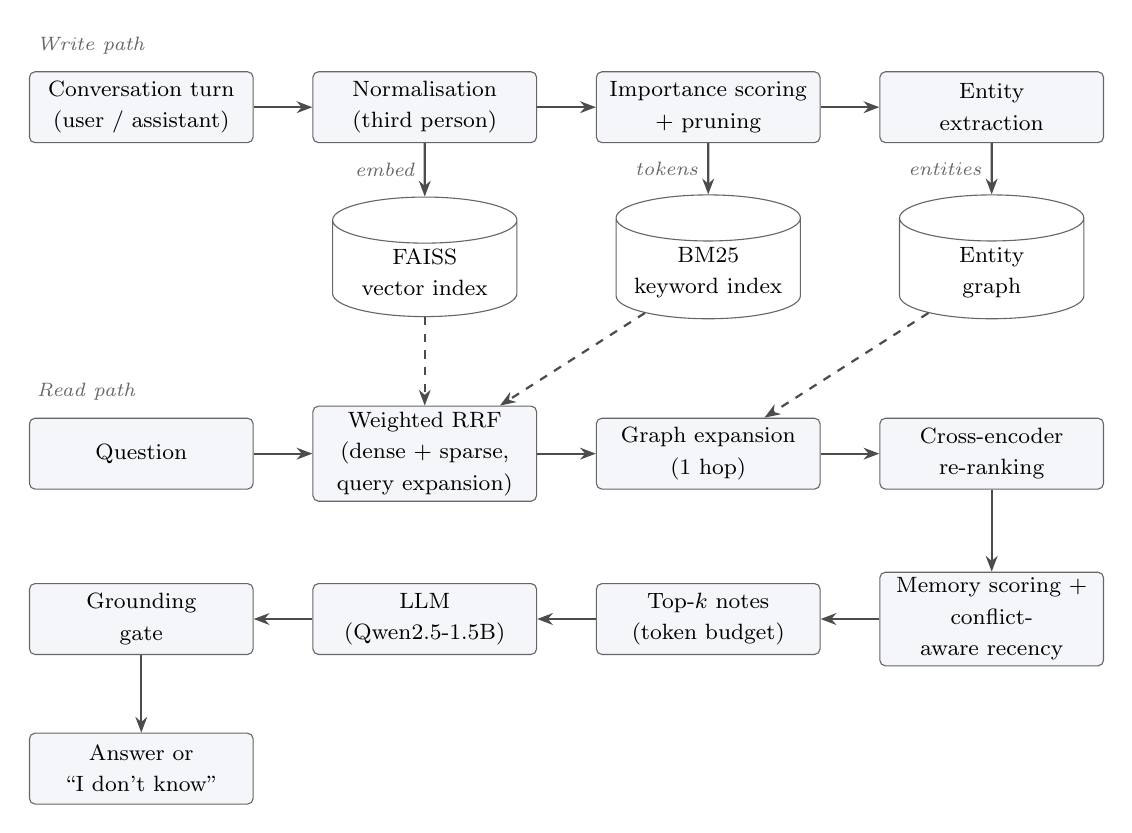
\begin{tikzpicture}[x=1cm,y=1cm,
  box/.style={draw=black!60,fill=boxfill,rounded corners=2pt,align=center,font=\footnotesize,
              minimum height=9mm,inner sep=2pt,text width=27mm},
  store/.style={draw=black!60,fill=white,cylinder,shape border rotate=90,aspect=0.25,align=center,
                font=\footnotesize,minimum height=10mm,text width=22mm,inner sep=2pt},
  lbl/.style={font=\scriptsize\itshape,text=black!60},
  arr/.style={-{Stealth[length=2mm]},thick,draw=black!70}
]
% ---- write path (top row) and the three stores
\node[box] (turn) at (0,0) {Conversation turn\\(user / assistant)};
\node[box] (norm) at (3.6,0) {Normalisation\\(third person)};
\node[box] (imp)  at (7.2,0) {Importance scoring\\$+$ pruning};
\node[box] (ent)  at (10.8,0) {Entity\\extraction};
\node[store] (vec) at (3.6,-2.1) {FAISS\\vector index};
\node[store] (bm)  at (7.2,-2.1) {BM25\\keyword index};
\node[store] (gr)  at (10.8,-2.1) {Entity\\graph};
\draw[arr] (turn) -- (norm); \draw[arr] (norm) -- (imp); \draw[arr] (imp) -- (ent);
\draw[arr] (norm) -- node[lbl,left]{embed} (vec);
\draw[arr] (imp)  -- node[lbl,left]{tokens} (bm);
\draw[arr] (ent)  -- node[lbl,left]{entities} (gr);
\node[lbl,anchor=south west] at (-1.45,0.55) {Write path};
% ---- read path, first row (left to right)
\node[box] (q)    at (0,-4.4) {Question};
\node[box] (fuse) at (3.6,-4.4) {Weighted RRF\\(dense $+$ sparse,\\query expansion)};
\node[box] (gx)   at (7.2,-4.4) {Graph expansion\\(1 hop)};
\node[box] (rr)   at (10.8,-4.4) {Cross-encoder\\re-ranking};
% ---- read path, second row (right to left)
\node[box] (sc)   at (10.8,-6.5) {Memory scoring $+$\\conflict-aware recency};
\node[box] (ctx)  at (7.2,-6.5) {Top-$k$ notes\\(token budget)};
\node[box] (llm)  at (3.6,-6.5) {LLM\\(Qwen2.5-1.5B)};
\node[box] (gate) at (0,-6.5) {Grounding\\gate};
\node[box] (ans)  at (0,-8.4) {Answer or\\``I don't know''};
\draw[arr] (q) -- (fuse); \draw[arr] (fuse) -- (gx); \draw[arr] (gx) -- (rr);
\draw[arr] (rr) -- (sc); \draw[arr] (sc) -- (ctx); \draw[arr] (ctx) -- (llm);
\draw[arr] (llm) -- (gate); \draw[arr] (gate) -- (ans);
\draw[arr,dashed] (vec) -- (fuse); \draw[arr,dashed] (bm) -- (fuse); \draw[arr,dashed] (gr) -- (gx);
\node[lbl,anchor=south west] at (-1.45,-3.85) {Read path};
\end{tikzpicture}
\caption{Architecture of the implemented memory layer. Dashed arrows are index look-ups.}
\label{fig:arch}
\end{figure}

\section{Data Acquisition and Benchmark Design}
\label{sec:data}
Public long-term memory benchmarks (LoCoMo, LongMemEval) are designed for large API models and do not give
ground-truth \emph{memory identifiers}, which we need to measure retrieval recall. We therefore generated a
controlled benchmark in the same spirit (\texttt{benchmarks/make\_dataset.py}). Each simulated user talks
to an assistant over 12 sessions of 12 user--assistant pairs (288 turns, about 3.6k tokens of history).
Into the small talk we insert:
\begin{itemize}[nosep]
  \item \textbf{10 single-hop personal facts} drawn from 18 attribute types (city, job, pet, allergy, doctor,
        laptop, \dots), each stated once with one of three paraphrases.
  \item \textbf{2 updated facts} (e.g.\ a move or a job change) stated in a later session, which create a
        \emph{temporal-current} question (``Where does the user live now?'') and a \emph{temporal-before}
        question (``Where did the user live before moving?'').
  \item \textbf{2 multi-hop chains} in which a related person is introduced in one session and a fact about
        that person appears in another (``My sister Priya visited'' $\rightarrow$ ``Priya adopted a cat named
        Milo'' $\rightarrow$ ``What did the user's sister name her cat?'').
  \item \textbf{8 distractor facts} about other people that reuse the attribute vocabulary (``My neighbour's
        dog is called Luna'') to punish lexical matching.
  \item \textbf{3 unanswerable questions} about attributes that were never mentioned; the correct answer is
        an abstention.
\end{itemize}
Questions are paraphrased relative to the stored statements, so a question rarely shares its exact wording
with its evidence. The test split contains 20 users and 330 questions (170 single-hop, 30 temporal-current,
30 temporal-before, 40 multi-hop, 60 unanswerable). A separate 6-user development split with a different
random seed was used for all hyper-parameter tuning. A second generator builds the NIAH-style histories of
1k--16k tokens used in Section~\ref{sec:niah}.

\section{Write Path}
\subsection{Memory Normalisation}
\label{sec:normalisation}
Questions are asked about ``the user'' while memories are written in the first person. Both the embedding
model and the cross-encoder treat ``I live in Pune'' and ``Where does the user live?'' as only weakly
related. Each turn is therefore rewritten into the third person at write time with a small set of pronoun
rules (``I'' $\rightarrow$ ``the user'', ``my'' $\rightarrow$ ``the user's'', assistant ``you'' $\rightarrow$
``the user''). On a probe set this raised the cosine similarity of question--memory pairs from about 0.3 to
0.6 and moved the cross-encoder logit of the correct memory from $-9$ (confidently irrelevant) to $+4$.

\subsection{Importance Scoring and Pruning}
Every turn receives an importance score in $[0,1]$ from cheap surface cues: user turns score higher than
assistant turns; statements that mention the speaker, contain a capitalised entity or a number, use
personal-fact vocabulary (\emph{live, work, named, allergic, birthday, deadline, \dots}) or are longer than
five words gain points, and questions lose points. A configurable threshold discards low-importance turns at
write time; Section~\ref{sec:pruning} shows that about 84\% of the turns can be discarded without any loss of
retrieval recall.

\subsection{Indexes and Entity Graph}
Each stored memory is embedded with \texttt{all-MiniLM-L6-v2} \cite{sbert} (384 dimensions, L2-normalised)
and inserted into a flat inner-product FAISS index \cite{faiss}; its stemmed, stop-word-filtered tokens are
added to a BM25 index \cite{bm25}; and its entities (capitalised names and product names, dates, numbers,
extracted with regular expressions and a sentence-initial filter) become nodes in a bipartite memory--entity
graph implemented with NetworkX. Entities linked to more than 25 memories are treated as hubs and ignored
during expansion.

\section{Read Path}
\subsection{Hybrid First Stage and Fusion}
\label{sec:fusion}
The question is embedded and the 20 nearest memories are fetched from FAISS. In parallel, the question is
expanded with a rule-based synonym table (\emph{city} $\rightarrow$ \emph{live, based, moved, home, \dots})
and the 20 best BM25 matches are fetched; BM25 hits scoring below 20\% of the best hit are discarded, which
removes near-zero ``matches'' caused by frequent words. The two lists are merged by weighted reciprocal
rank fusion \cite{rrf}
\[
  s_{\text{fused}}(m) = \sum_{c \in \{\text{dense},\,\text{sparse}\}} \frac{w_c}{k + \text{rank}_c(m)},
  \qquad k = 60,\; w_{\text{dense}} = 1,\; w_{\text{sparse}} = 0.2 .
\]
The sparse weight was chosen on the development split: with equal weights the weak lexical channel reduced
recall below that of dense retrieval alone.

\subsection{Entity-Graph Expansion}
The top-3 fused candidates act as seeds. Every memory that shares a non-hub entity with a seed inherits
$0.85\times$ the seed's fused score (one-step relevance propagation); at most four such memories are added
to the candidate pool. This is how the second hop of a chain question enters the pool: ``Dev started working
at Zoho'' never mentions a brother, but it shares the entity \emph{Dev} with ``The user's brother Dev lives
with the user'', which the first stage finds easily.

\subsection{Cross-Encoder Re-ranking}
Up to 40 candidates are scored jointly with the question by the MS~MARCO MiniLM-L6 cross-encoder
\cite{nogueira2019}. Because the cross-encoder was found to be unreliable on its own for these short
conversational notes, its sigmoid output is blended with the normalised fused score,
$\text{rel}(m) = 0.5\,\sigma(\text{CE}(m)) + 0.5\, s_{\text{fused}}(m)/\max s_{\text{fused}}$.

\subsection{Memory Scoring}
\label{sec:scoring}
Following the memory-stream idea \cite{park2023}, each candidate is scored with relevance, recency,
importance, access frequency and a graph-coherence bonus (number of other candidates it shares an entity
with). Unlike the additive formulation, relevance acts as a gate:
\[
  \text{score}(m) = \text{rel}(m)\,\bigl(1 + w_{\text{rec}}\,2^{-\Delta s/h} + w_{\text{imp}}\,\text{imp}(m)
  + w_{\text{acc}}\,\text{acc}(m) + w_{\text{graph}}\,\text{coh}(m)\bigr),
\]
with $\Delta s$ the age in sessions and half-life $h = 6$. On the development split a non-zero recency
weight lowered recall for multi-hop and ``before'' questions, so recency is applied through the conflict
rule below instead ($w_{\text{rec}} = 0$, $w_{\text{imp}} = 0.10$, $w_{\text{acc}} = 0.02$,
$w_{\text{graph}} = 0.10$). Finally, a memory that is itself a question or request to the assistant
(``What is a good way to learn guitar chords?'') is multiplied by $0.7$: such turns are rarely evidence for
a fact about the user, yet they match question words such as \emph{learning} very well. This single rule
raised single-hop Recall@5 from 92\% to 99\% on the test split without affecting the other question types.

\subsection{Conflict-Aware Recency (Memory Updates)}
Two candidates are treated as versions of the same fact when both are user statements about the user (no
third-party nouns such as \emph{colleague} or \emph{neighbour}), their cosine similarity is at least 0.45 and
the newer one contains an update cue (\emph{moved, switched, upgraded, replaced, now, new, \dots}). The older
version keeps 80\% of its score and is tagged ``(older note)'' when injected, so the LLM can still answer
``before'' questions while being steered to the current fact.

\subsection{Context Injection and Grounding Gate}
The top-5 memories are rendered chronologically with their session label inside a 512-token budget, and the
LLM is instructed to answer only from the notes, to prefer the most recent note when notes conflict, to
ignore notes about other people, and to reply ``I don't know'' otherwise. After generation the
\emph{grounding gate} verifies the answer: the note whose content covers the answer's content words is
located, and the answer is accepted only if that note's relevance score is at least 0.35. An answer copied
from an irrelevant note (the neighbour's dog) or not found in any note is replaced by an abstention. This
gate is the Phase-2 counterpart of the hallucination detectors evaluated in Phase 1.

\section{Baselines and Evaluation Protocol}
All strategies use the same model, Qwen2.5-1.5B-Instruct \cite{qwen25} in fp16 on a 4~GB laptop GPU, with
greedy decoding, the same system prompt and the same answer-format instructions:
\begin{itemize}[nosep]
  \item \textbf{Baseline LLM}: question only, no memory.
  \item \textbf{Full context}: the complete transcript of all sessions in the prompt (the context-window
        expansion approach; prompts up to 16k tokens use chunked prefill so that they fit in GPU memory).
  \item \textbf{Sliding window}: the last 40 turns.
  \item \textbf{Vector RAG}: the Phase-1 design, embedding similarity top-5 only.
  \item \textbf{Memory layer}: the full pipeline above, reported with and without the grounding gate.
\end{itemize}
An answer is correct when the normalised gold string is contained in it or token-F1 $\ge 0.6$; an
unanswerable question is correct only when the model abstains. A \emph{hallucination} is a non-abstaining
answer that is wrong, or any non-abstaining answer to an unanswerable question. For retrieval methods we also
report Recall@$k$ (all gold memories within the top-$k$) and MRR. Latency and prompt tokens are measured per
question. The implementation is about 2,400 lines of Python: the package \texttt{memory\_layer} (eleven modules),
the \texttt{benchmarks} directory (dataset generator, three experiment runners, tuning and plotting) and a
functional test suite; all experiments are reproducible from the committed scripts.


\chapter{Simulation and Results}
\label{ch:result}

\section{Overview of Experimental Setup}
All experiments were run on a laptop with an NVIDIA RTX~3050 (4~GB) GPU and 16 CPU threads. The answering
model is \llmName{} in fp16 with greedy decoding; the embedding model is all-MiniLM-L6-v2 and the re-ranker
is the MS~MARCO MiniLM-L6 cross-encoder. Four experiments were carried out:
\begin{enumerate}[nosep]
  \item \textbf{Main comparison} (Section~\ref{sec:main}): five answering strategies on the \nUsers-user,
        \nQuestions-question test split described in Section~\ref{sec:data}.
  \item \textbf{Hallucination analysis} (Section~\ref{sec:halluc}): hallucination rates of every strategy
        and the precision/recall of the grounding gate, compared with the Phase-1 detectors.
  \item \textbf{Retrieval ablation} (Section~\ref{sec:ablation}): each pipeline stage switched on in turn,
        plus pruning and conflict-threshold sweeps, measured with retrieval metrics (no LLM).
  \item \textbf{Context-length scaling} (Section~\ref{sec:niah}): the needle-in-a-haystack protocol of
        Phase 1, now run on our own hardware with histories from 1k to \niahMaxLen{} tokens.
\end{enumerate}
All hyper-parameters were fixed on the separate development split before the test split was evaluated.

\section{Main Comparison of Answering Strategies}
\label{sec:main}
Table~\ref{tab:main} and Figure~\ref{fig:main} summarise the end-to-end results.
\begin{table}[htbp]\centering\small\resizebox{\textwidth}{!}{%
\begin{tabular}{lccccc}\hline
\textbf{Method} & \textbf{Accuracy} & \textbf{Acc. (answerable)} & \textbf{Halluc. rate} & \textbf{Abstain (unans.)} & \textbf{Prompt tokens}\\\hline
Baseline LLM (no memory) & 18.2\% & 0.0\% & 0.0\% & 100.0\% & 117\\
Full context (whole history) & 57.3\% & 61.1\% & 36.1\% & 40.0\% & 4,209\\
Sliding window (last 40 turns) & 26.4\% & 11.1\% & 11.2\% & 95.0\% & 664\\
Vector RAG (Phase-1 design) & 73.6\% & 73.3\% & 17.9\% & 75.0\% & 266\\
\textbf{Memory layer (proposed)} & \textbf{78.2\%} & \textbf{80.0\%} & \textbf{15.5\%} & \textbf{70.0\%} & \textbf{267}\\
\textbf{Memory layer + grounding gate} & \textbf{80.6\%} & \textbf{79.3\%} & \textbf{7.0\%} & \textbf{86.7\%} & \textbf{267}\\
\hline\end{tabular}}
\caption{End-to-end comparison on the long-term conversational memory benchmark (20 users, 330 questions, Qwen2.5-1.5B-Instruct).}
\label{tab:main}\end{table}


\begin{figure}[htbp]\centering
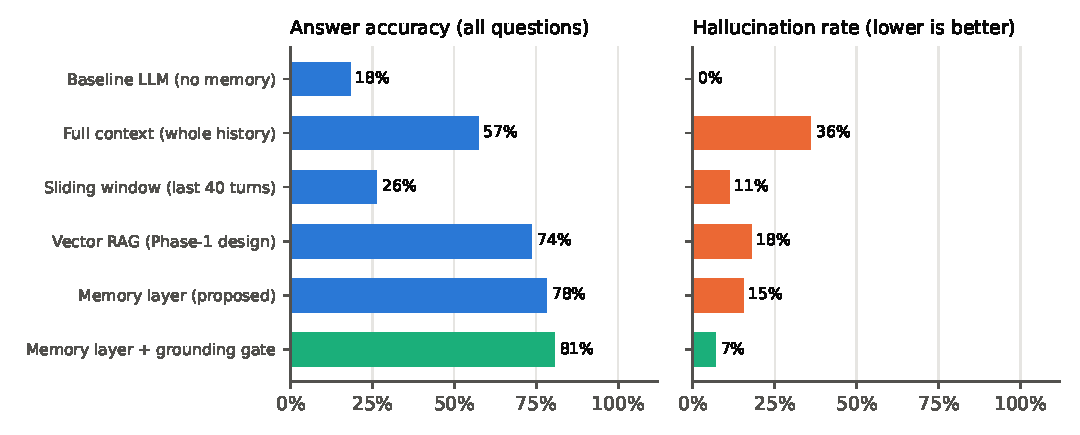
\includegraphics[width=\textwidth]{fig_main_accuracy.pdf}
\caption{Answer accuracy and hallucination rate of the five answering strategies (test split).}
\label{fig:main}
\end{figure}

\textbf{Baseline LLM.} Without any memory the model answers \accNone\% of the questions, and all of those
are unanswerable questions on which it correctly says ``I don't know''. It never guesses a personal fact,
so its hallucination rate is \halNone\%, but it is useless for the task: accuracy on answerable questions
is \accAnsNone\%.

\textbf{Full context.} Sending the entire history (\tokFull{} tokens per query on average) recovers
\accFull\% accuracy, but it also produces the highest hallucination rate of all strategies, \halFull\%. With
288 turns in the prompt, eight of which are distractor facts about other people, the model frequently
returns the neighbour's dog or the colleague's city, and it confuses old and current facts. This is the
Phase-1 finding reproduced with our own model and data: a longer context is not a reliable memory.

\textbf{Sliding window.} The last 40 turns cost \tokWin{} tokens and give only \accWin\% accuracy, because
almost every fact was stated in an earlier session. Its low hallucination rate (\halWin\%) is simply the
result of abstaining most of the time.

\textbf{Vector RAG (Phase-1 design).} Embedding search alone is already a large improvement: \accRag\%
accuracy with \tokRag{} tokens per query, i.e.\ \tokRatioFullMem$\times$ fewer tokens than the full
context and a higher accuracy. Its retrieval recall@5 is \recRag\%.

\textbf{Memory layer.} The full pipeline raises recall@5 to \recMem\% and accuracy to \accMem\%
(\accAnsMem\% on answerable questions) at the same token cost, and lowers the hallucination rate to
\halMem\%. With the grounding gate the hallucination rate halves again to \halMemGate\% while accuracy
rises to \accMemGate\%, because answers copied from a note about the wrong person are converted into
abstentions, which are the correct response for the unanswerable questions (abstention rate
\absMemGate\% versus \absMem\% without the gate).

\section{Accuracy by Question Type}
Table~\ref{tab:types} and Figure~\ref{fig:types} break the accuracy down by question type, which shows
\emph{where} the memory layer differs from plain vector RAG.
\begin{table}[htbp]\centering\small\resizebox{\textwidth}{!}{%
\begin{tabular}{lccccc}\hline
\textbf{Method} & \textbf{Single-hop} & \textbf{Temporal (current)} & \textbf{Temporal (before)} & \textbf{Multi-hop} & \textbf{Unanswerable}\\\hline
Full context (whole history) & 62.4\% & 80.0\% & 13.3\% & 77.5\% & 40.0\%\\
Sliding window (last 40 turns) & 10.0\% & 30.0\% & 0.0\% & 10.0\% & 95.0\%\\
Vector RAG (Phase-1 design) & 80.6\% & 86.7\% & 50.0\% & 50.0\% & 75.0\%\\
Memory layer (proposed) & 81.2\% & 90.0\% & 63.3\% & 80.0\% & 70.0\%\\
\hline\end{tabular}}
\caption{Accuracy by question type.}\label{tab:types}\end{table}


\begin{figure}[htbp]\centering
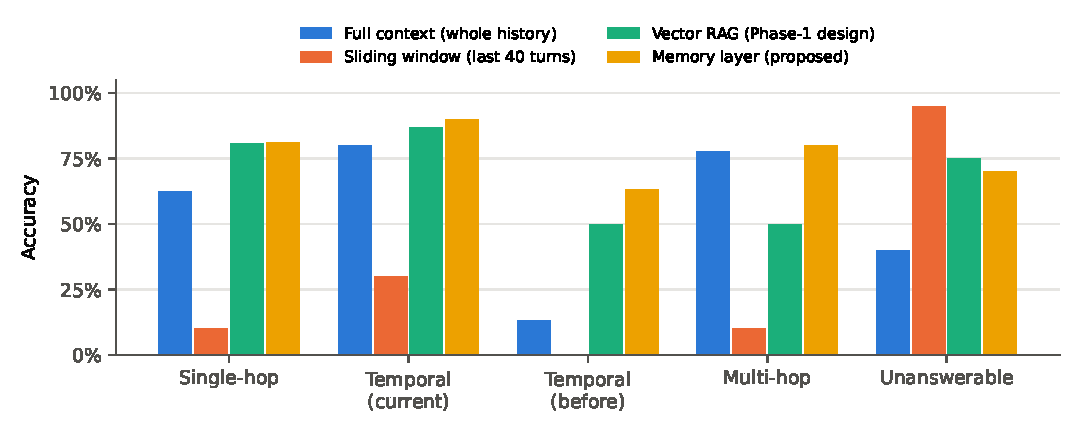
\includegraphics[width=\textwidth]{fig_type_accuracy.pdf}
\caption{Accuracy by question type for the four context-based strategies.}
\label{fig:types}
\end{figure}

\begin{itemize}[nosep]
  \item \textbf{Multi-hop} questions are where the entity graph pays off: \accMemMH\% for the memory
        layer against \accRagMH\% for vector RAG. Vector search finds the note that introduces the
        relative but not the note about that relative, which never mentions the relation word.
  \item \textbf{Temporal (before)} questions improve from \accRagTB\% to \accMemTB\%: the conflict rule
        keeps the old version of a fact in the prompt and tags it as an older note, so the model can
        answer ``where did the user live before moving''. The full-context baseline reaches only
        \accFullTB\% here: with both statements thousands of tokens apart it almost always returns the
        current value.
  \item \textbf{Temporal (current)} questions are answered similarly by the two retrieval methods
        (\accRagTC\% and \accMemTC\%) and by the full context (\accFullTC\%); the chronological rendering
        and the ``trust the most recent note'' instruction already handle most updates.
  \item \textbf{Single-hop} questions are answered correctly \accMemSH\% of the time by the memory layer
        and \accRagSH\% by vector RAG. Retrieval recall is above 97\% for both, so the remaining errors are
        generation errors of the 1.5B model in the presence of distractor notes.
  \item \textbf{Unanswerable} questions are the weak point of every retrieval method without the gate:
        when nothing relevant exists, the retriever still returns five notes and the small model is
        tempted to answer from them. The grounding gate raises abstention on these questions to
        \absMemGate\%.
\end{itemize}

\section{Hallucination Analysis and the Grounding Gate}
\label{sec:halluc}
In Phase 1 the hallucination detectors available for RAG outputs (Table~4.1 of the Phase-1 report)
reached recall of 0.88--0.95 but precision of only 0.25--0.26: they flagged almost everything. The
Phase-2 grounding gate takes the opposite approach. It does not try to judge fluency or plausibility;
it checks three deterministic properties of the answer against the injected notes: is the answer
attributable to a note, is that note a statement rather than a request, and is the note about the same
subject as the question. Table~\ref{tab:halluc} compares the two phases on their respective data.
\begin{table}[htbp]\centering\small
\begin{tabular}{lccc}\hline
\textbf{Detector} & \textbf{Precision} & \textbf{Recall} & \textbf{F1}\\\hline
Phase 1: Mistral 7B (RAGTruth) & 0.25 & 0.92 & 0.39\\
Phase 1: Llama 2 (RAGTruth) & 0.26 & 0.95 & 0.41\\
Phase 1: TinyLlama (RAGTruth) & 0.25 & 0.88 & 0.38\\\hline
Phase 2: grounding gate on vector RAG & 0.89 & 0.42 & 0.57\\
Phase 2: grounding gate on memory layer & 0.93 & 0.55 & 0.69\\
\hline\end{tabular}
\caption{Hallucination detection: Phase-1 results versus the Phase-2 grounding gate.}\label{tab:halluc}\end{table}


On the memory layer's answers the gate flags \gateFlaggedMem{} of \nQuestions{} answers, of which
\gateTPMem{} are indeed hallucinations (precision \gatePMem); it misses \gateFNMem{} of the
\gatePosMem{} hallucinations, mostly answers that copy the \emph{wrong user fact} (e.g.\ the user's
company when asked for the gym), which are attributable, factual and about the user and therefore pass all
three checks (recall \gateRMem). The resulting F1 of \gateFMem{} is substantially above the 0.38--0.41 of the Phase-1
detectors, and, unlike those detectors, the gate costs no additional model call. Applied to the vector-RAG
pipeline the same gate reaches F1 \gateFRag, so the gain is not specific to our retriever.

The hallucination rate of the complete system (memory layer with gate) is \halMemGate\% over all
questions and \halAnsMemGate\% on answerable questions, compared with \halFull\% for the full-context
approach and \halRag\% for plain vector RAG.

\section{Retrieval Ablation}
\label{sec:ablation}
Table~\ref{tab:ablation} and Figure~\ref{fig:ablation} switch the pipeline stages on one at a time and
report retrieval quality on the 270 answerable test questions. Recall@$k$ requires \emph{all} gold
memories of a question to be in the top-$k$ (two for multi-hop questions).
\begin{table}[htbp]\centering\small
\begin{tabular}{lccccc}\hline
\textbf{Configuration} & \textbf{R@1} & \textbf{R@3} & \textbf{R@5} & \textbf{MRR} & \textbf{Temporal ok}\\\hline
Vector only & 58.9\% & 86.3\% & 90.4\% & 0.829 & 70.0\%\\
BM25 only & 24.1\% & 41.1\% & 43.7\% & 0.439 & 26.7\%\\
+ RRF hybrid & 48.9\% & 79.6\% & 87.4\% & 0.756 & 65.0\%\\
+ query exp. & 54.8\% & 80.0\% & 89.6\% & 0.794 & 61.7\%\\
+ re-ranking & 54.1\% & 84.1\% & 88.9\% & 0.801 & 60.0\%\\
+ entity graph & 54.1\% & 84.8\% & 90.7\% & 0.801 & 60.0\%\\
+ scoring (full) & 56.7\% & 88.9\% & 96.3\% & 0.827 & 80.0\%\\
\hline\end{tabular}
\caption{Retrieval ablation: each row adds one stage to the previous one. R@k = all gold memories within the top-k; Temporal ok = the current fact outranks the outdated one.}\label{tab:ablation}\end{table}


\begin{figure}[htbp]\centering
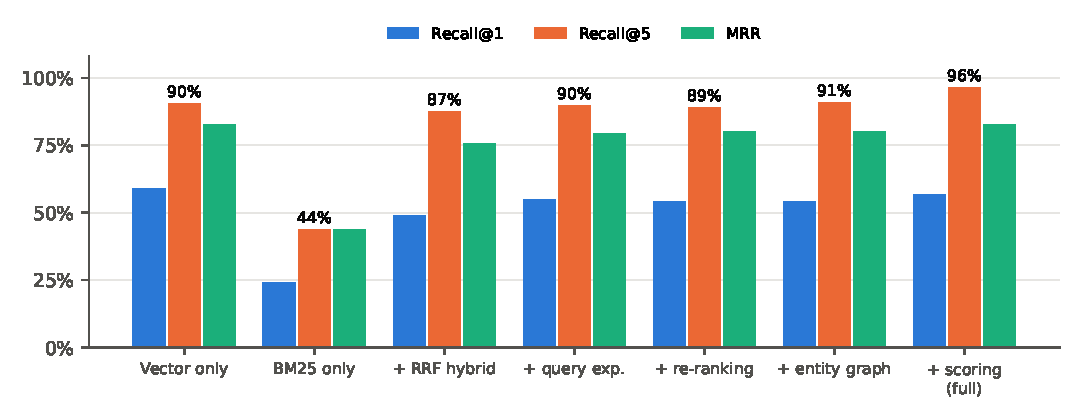
\includegraphics[width=\textwidth]{fig_ablation.pdf}
\caption{Retrieval quality as pipeline stages are added. Each configuration includes all stages to its left.}
\label{fig:ablation}
\end{figure}

\begin{figure}[htbp]\centering
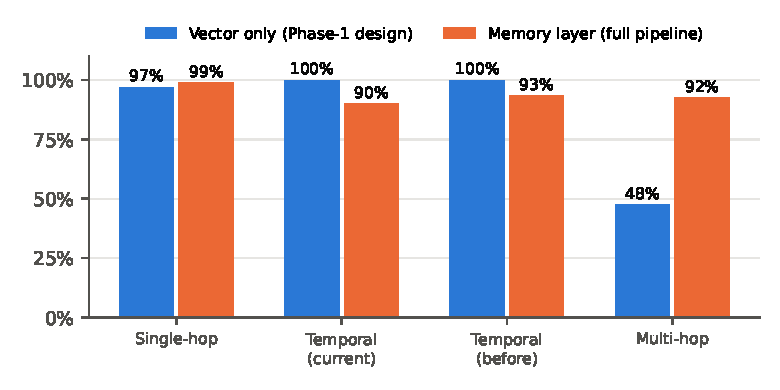
\includegraphics[width=0.78\textwidth]{fig_ablation_types.pdf}
\caption{Recall@5 by question type: Phase-1 vector-only retrieval versus the full memory layer.}
\label{fig:ablation_types}
\end{figure}

Three observations stand out. First, \textbf{BM25 on its own is poor} (\rFiveBm\% recall@5) because the
questions are paraphrases of the stored statements, and fusing the raw lexical ranking with the dense one
\emph{lowers} recall below dense retrieval alone (\rFiveHyb\% vs.\ \rFiveVec\%); only with query
expansion does the lexical channel stop hurting (\rFiveQe\%), and it starts paying off once the later
stages can exploit the exact-match candidates it contributes. Second, the
\textbf{entity graph} is the stage that changes the picture for multi-hop questions:
recall@5 on them goes from \rFiveVecMH\% for vector-only retrieval to \rFiveMemMH\% for the full layer
(Figure~\ref{fig:ablation_types}), with almost no cost on single-hop questions (\rFiveVecSH\% vs.\
\rFiveMemSH\%). Third, \textbf{memory scoring and the question penalty} add the final points: overall
recall@5 rises from \rFiveVec\% (Phase-1 design) to \rFiveMem\%, and the share of temporal questions whose
current version outranks the outdated one rises from \tempVec\% to \tempMem\%.

\section{Importance-Based Pruning and the Conflict Threshold}
\label{sec:pruning}
Table~\ref{tab:pruning} and Figure~\ref{fig:pruning} vary the write-time importance threshold $\theta$.
Keeping only turns with importance $\ge 0.3$ stores \pruneKeptThree\% of the turns and still achieves
\pruneRecThree\% recall@5 (\pruneRecZero\% with everything stored); the discarded turns are generic
assistant replies and short small talk. At $\theta = 0.45$ only \pruneKeptFortyFive\% of the turns remain
for a recall of \pruneRecFortyFive\%, a loss of under four points for a six-fold smaller store, and above
$\theta = 0.5$ genuine facts start to be dropped and recall falls quickly. The importance heuristic
therefore separates facts from chatter well enough to halve the memory store at no cost, and the
threshold gives an explicit storage/recall trade-off.
\begin{table}[htbp]\centering\small
\begin{tabular}{lccc}\hline
\textbf{Importance threshold $\theta$} & \textbf{Memories kept} & \textbf{R@5} & \textbf{MRR}\\\hline
0.0 & 100.0\% & 96.3\% & 0.827\\
0.3 & 55.5\% & 95.9\% & 0.811\\
0.45 & 16.9\% & 92.6\% & 0.779\\
0.55 & 9.6\% & 80.4\% & 0.695\\
0.65 & 6.8\% & 76.3\% & 0.658\\
\hline\end{tabular}
\caption{Write-time pruning: fraction of turns kept as memories and the resulting retrieval quality.}\label{tab:pruning}\end{table}


\begin{figure}[htbp]\centering
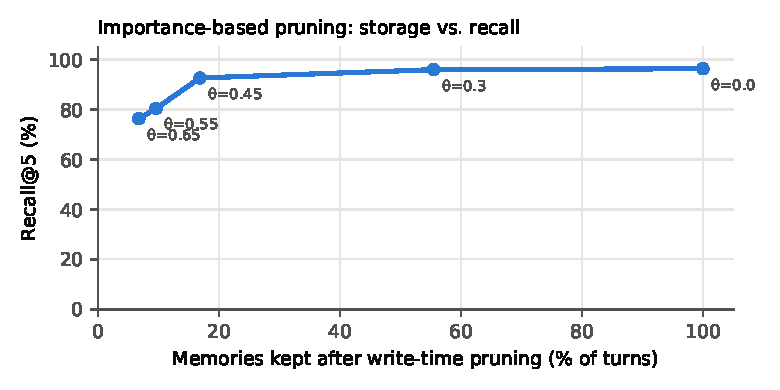
\includegraphics[width=0.72\textwidth]{fig_pruning.pdf}
\caption{Write-time pruning: fraction of turns kept versus retrieval recall for different thresholds.}
\label{fig:pruning}
\end{figure}

The conflict-threshold sweep shows the expected trade-off: a low cosine threshold (0.3) tags more pairs as
old/new versions and gives the best temporal ordering, but also tags unrelated facts and slightly lowers
overall recall; the dev-selected value of 0.45 keeps overall recall at its maximum while still ordering
\tempMem\% of temporal questions correctly.

\section{Context-Length Scaling (Needle in a Haystack)}
\label{sec:niah}
Phase 1 quoted needle-in-a-haystack results from the literature. Here the protocol was run on our own
model: a single personal fact is placed at one of five depths inside a filler conversation of 1k to
\niahMaxLen{} tokens (plus six distractor facts), and the model is asked about it either from the full
transcript or from the memory layer's top-5 notes (\niahNeedles{} needles per cell, \niahCells{} cells).
Table~\ref{tab:niah} and Figures~\ref{fig:niah} and~\ref{fig:niah_heat} give the results.
\begin{table}[htbp]\centering\small
\begin{tabular}{lcccccc}\hline
\textbf{History length} & \multicolumn{3}{c}{\textbf{Full context}} & \multicolumn{3}{c}{\textbf{Memory layer}}\\
 & Acc. & Tokens & Latency & Acc. & Tokens & Latency\\\hline
1k & 82\% & 1,080 & 1.11s & 90\% & 270 & 0.65s\\
2k & 82\% & 2,096 & 1.85s & 92\% & 265 & 0.66s\\
4k & 85\% & 4,184 & 3.03s & 80\% & 264 & 0.68s\\
8k & 75\% & 8,335 & 6.23s & 82\% & 263 & 0.67s\\
16k & 75\% & 16,634 & 81.64s & 72\% & 267 & 0.70s\\
\hline\end{tabular}
\caption{Needle-in-a-haystack scaling: accuracy, prompt size and latency versus history length.}\label{tab:niah}\end{table}


\begin{figure}[htbp]\centering
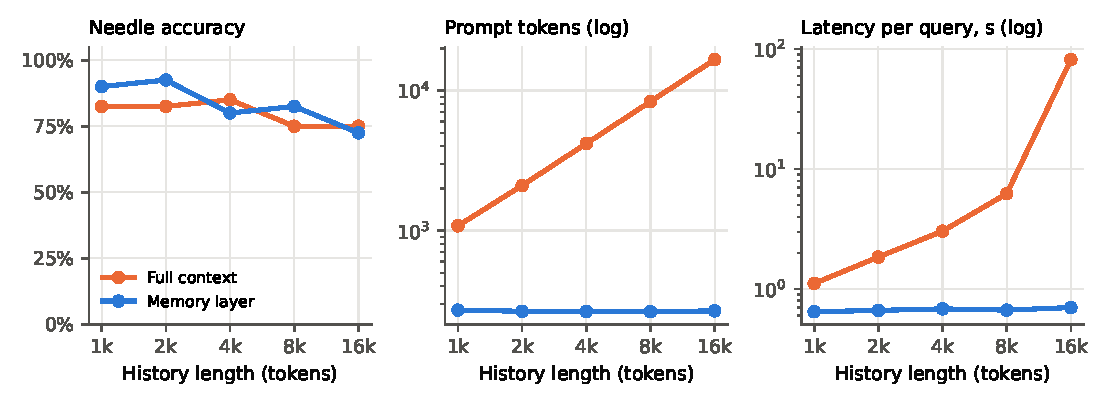
\includegraphics[width=\textwidth]{fig_niah_lines.pdf}
\caption{Needle accuracy, prompt size and latency versus history length for full-context prompting and
the memory layer.}
\label{fig:niah}
\end{figure}

\begin{figure}[htbp]\centering
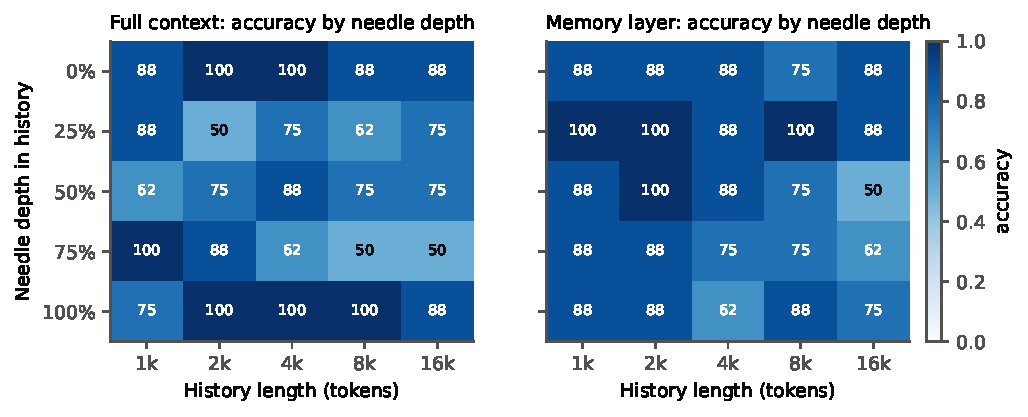
\includegraphics[width=\textwidth]{fig_niah_heatmap.pdf}
\caption{Accuracy by needle depth and history length (the Phase-2 counterpart of the Phase-1 NIAH heatmap).}
\label{fig:niah_heat}
\end{figure}

Two things are visible. The memory layer's prompt stays at about \niahTokMemLast{} tokens whatever the
history length, while the full-context prompt grows to \niahTokFullLast{} tokens at \niahMaxLen{}
(\niahTokRatioLast$\times$ more); latency grows accordingly, from \niahLatFullFirst{}~s to
\niahLatFullLast{}~s per query for the full context against \niahLatMemLast{}~s for the memory layer at
\niahMaxLen{} tokens (\niahLatRatioLast$\times$ faster). On this single-needle task the 1.5B model's
accuracy from the full context is \niahFullAccFirst\% at 1k and \niahFullAccLast\% at \niahMaxLen{}
tokens (mean \niahFullAccMean\%), while the memory layer gives \niahMemAccFirst\% and \niahMemAccLast\%
(mean \niahMemAccMean\%) with the needle retrieved into the top-5 in \niahMemRecallMean\% of cases.
At \niahMaxLen{} tokens the memory layer holds \niahMemMemories{} notes; the needle is still retrieved
93\% of the time, so its lower accuracy there is again a reading error of the small model, which has to
pick the needle out of five notes that now include more same-attribute distractors.
The important contrast with Section~\ref{sec:main} is that a \emph{single} needle in filler text is a
much easier problem than a real multi-session history: the full-context model degrades far more when the
haystack contains many similar facts, updates and distractors (\accFull\% there) than when it contains
one fact among small talk. The difficulty of long-context memory is interference, not length alone, and
retrieval of a few verified notes removes the interference while keeping the cost constant.

\section{Efficiency: Tokens and Latency}
Figure~\ref{fig:tokens} compares prompt size and end-to-end latency on the main benchmark. The memory
layer sends \tokMem{} tokens per query against \tokFull{} for the full context
(\tokRatioFullMem$\times$ fewer) and answers in \latMem{}~s against \latFull{}~s
(\latRatioFullMem$\times$ faster). The retrieval stages themselves (embedding the question, FAISS and
BM25 look-ups, graph expansion, cross-encoder re-ranking and scoring) take 30--50~ms per query on the
GPU and about 30~ms on the CPU, against 6~ms for plain vector search; the rest of the latency is LLM
generation. Ingesting a complete 288-turn history (normalisation, embedding, indexing and entity
extraction) takes well under a second, and a 1,118-note history about a quarter of a second.

\begin{figure}[htbp]\centering
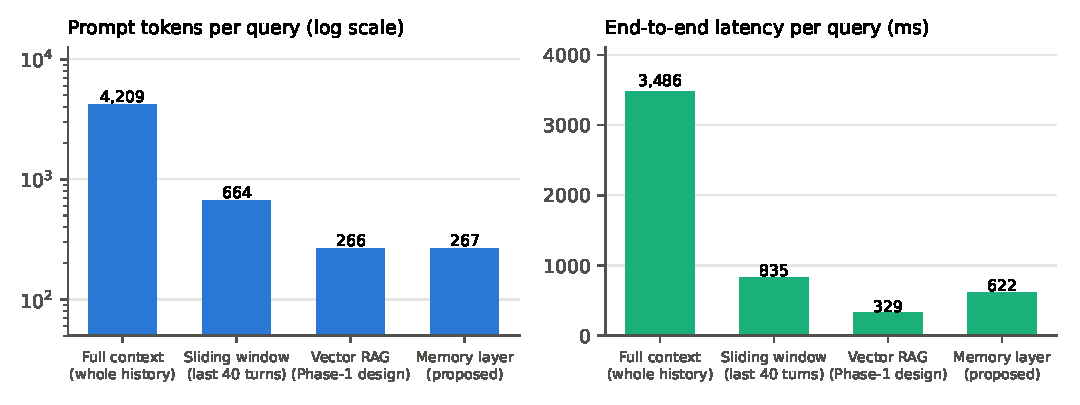
\includegraphics[width=\textwidth]{fig_tokens_latency.pdf}
\caption{Prompt tokens and end-to-end latency per query on the main benchmark.}
\label{fig:tokens}
\end{figure}

\section{Qualitative Example}
Listing~\ref{lst:trace} shows an actual trace of the memory layer on a short three-session history
(run on the CPU, hence the higher latencies). Note the third-person normalisation of the stored notes, the
``(older note)'' tag on the superseded city, the second-hop note (``Priya adopted a cat \dots'') reached
through the entity \emph{Priya}, and the abstention produced by the gate when the model answers the
car question from the note about the colleague. The second question also shows the typical residual error
of the small model: both the old and the new city are in the prompt, correctly labelled, yet it answers
with the current one.
\lstinputlisting[caption={Trace of the memory layer on a three-session history (verbatim program output).},
  label={lst:trace}]{example_trace.txt}

\section{Key Insights}
\begin{itemize}[nosep]
  \item A long context window is the \emph{worst} memory in the presence of updates and distractors: the
        full-context baseline hallucinates \halFull\% of the time, more than any other strategy.
  \item Selective retrieval is the main source of the gain (vector RAG alone reaches \accRag\%); the
        additional stages of the memory layer matter for the question types that vector search cannot
        solve: multi-hop (\accRagMH\% $\rightarrow$ \accMemMH\%) and temporal-before
        (\accRagTB\% $\rightarrow$ \accMemTB\%).
  \item Verification is as important as retrieval: the grounding gate halves the hallucination rate
        (\halMem\% $\rightarrow$ \halMemGate\%) with precision \gatePMem, where the Phase-1 detectors had
        precision 0.25.
  \item Memory can be pruned at write time: half of the turns carry all of the recall, and a sixth of
        them carry 96\% of it.
  \item The remaining errors are mostly generation errors of the small model, not retrieval errors
        (recall@5 \recMem\% versus accuracy \accMem\%), which points to a larger answering model or a
        reader fine-tuned on memory notes as the next step.
\end{itemize}


\chapter{Conclusions and Future Work}
\label{ch:conclude}

\section{Conclusion}
Phase 1 of this project analysed why Large Language Models struggle with long interactions: they are
stateless, their effective context is much shorter than their nominal window, and retrieval alone does
not stop hallucination. It proposed a persistent memory layer as the remedy. Phase 2 built that layer and
measured it.

The implemented system stores every conversation turn as a normalised, third-person note with an
importance score, an embedding, BM25 tokens and extracted entities. At query time it fuses dense and
lexical retrieval, expands candidates one hop through the entity graph, re-ranks them with a
cross-encoder, scores them with relevance-gated recency/importance/coherence terms, resolves conflicting
versions of a fact in favour of the newest one, injects the top five notes into a 512-token prompt and
finally verifies the generated answer against those notes.

On a \nQuestions-question long-term conversational benchmark, answered by the same 1.5B-parameter local
model under every strategy, the memory layer with its grounding gate reached \accMemGate\% accuracy with a
hallucination rate of \halMemGate\%, compared with \accFull\% and \halFull\% for sending the full
conversation history, \accRag\% and \halRag\% for the Phase-1 vector-RAG design, and \accWin\% for a
sliding window of recent turns. It did so with \tokMem{} prompt tokens per query, \tokRatioFullMem{} times
fewer than the full context, and \latRatioFullMem{} times lower latency. The stage-wise ablation showed
where the gains come from: the entity graph lifted multi-hop retrieval recall from \rFiveVecMH\% to
\rFiveMemMH\%, the conflict rule kept both versions of updated facts available, and the question penalty
removed small-talk turns that lexically resemble questions. Importance-based pruning showed that the memory
store can be halved without loss of recall, or reduced to a sixth of the turns at a cost of under four
recall points. The grounding gate, a set of
three deterministic evidence checks, detected hallucinations with precision \gatePMem{} and F1 \gateFMem,
against precision 0.25 and F1 0.39 for the detectors examined in Phase 1, at zero additional model cost.

The context-length experiment reproduced on our own hardware what Phase 1 took from the literature: the
cost of the full-context approach grows linearly with history length (\niahTokFullLast{} tokens and
\niahLatFullLast{}~s per query at \niahMaxLen{} tokens) while the memory layer stays constant
(\niahTokMemLast{} tokens, \niahLatMemLast{}~s). More importantly, the main benchmark showed that the real
difficulty of long-term memory is not length but \emph{interference} between many similar, updated and
unrelated facts, and that selecting a few verified notes removes that interference.

Taken together, the two phases support the thesis set out at the start of the project: a persistent,
selective and verified memory layer is a better foundation for long-running LLM applications than a larger
context window, and it can be built from standard, inexpensive components.

\section{Limitations}
\begin{itemize}[nosep]
  \item The benchmark is synthetic. It is controlled and reproducible, and it follows the LoCoMo and
        LongMemEval question taxonomy, but its conversations are simpler than real ones.
  \item The answering model is small (1.5B parameters). Retrieval recall is above 96\% while accuracy is
        about \accMem\%; most of the remaining errors are reading errors that a larger model would avoid.
  \item Entity extraction, importance scoring, query expansion and conflict detection are rule-based. They
        are free and transparent, but they only capture surface patterns.
  \item Hyper-parameters were tuned on a development split generated by the same generator; transfer to
        other domains would need re-tuning.
\end{itemize}

\section{Future Work}
\subsection{Write-Time Fact Extraction}
Replace the raw turn with LLM-extracted atomic facts (as in Mem0) so that a single turn containing two facts
becomes two memories, and so that the conflict rule can compare facts rather than sentences. The
extraction can be batched off-line, keeping query latency unchanged.

\subsection{Learned Components}
Fine-tune the cross-encoder on (question, memory note) pairs from the benchmark so that re-ranking is
reliable on conversational text, and train a light classifier for importance and for the
\emph{about-the-user} decision that the gate currently makes with regular expressions.

\subsection{Typed Entity Graph}
Extend the memory--entity graph with relation types (\emph{sister-of}, \emph{works-at},
\emph{lives-in}) so that multi-hop questions can be answered by typed traversal rather than one-hop
expansion, and so that an update of a relation (a move) can retire the old edge explicitly.

\subsection{Consolidation and Forgetting}
Periodically merge related notes into summaries and apply the Ebbinghaus-style decay of MemoryBank to
notes that are never accessed, keeping the store bounded for conversations that run for years.

\subsection{Evaluation on Public Benchmarks and Larger Models}
Run the layer on LoCoMo and LongMemEval with 7B--70B models to confirm that the gains transfer, and
measure the trade-off between answering-model size and memory-layer sophistication.

\subsection{Deployment}
Package the layer as a service with per-user isolation, encryption of stored notes, a right-to-forget
operation, and a web demo in which the retrieved notes and the gate decision are shown next to each
answer so that users can audit what the assistant remembers.

%% ----------------------------------------------------------------

\newpage

\addcontentsline{toc}{chapter}{Bibliography}

\begin{thebibliography}{99}

\bibitem{vaswani2017} A.~Vaswani et al., ``Attention Is All You Need,'' \emph{Advances in Neural Information
Processing Systems}, 2017.

\bibitem{lewis2020} P.~Lewis et al., ``Retrieval-Augmented Generation for Knowledge-Intensive NLP Tasks,''
\emph{NeurIPS}, 2020.

\bibitem{gao2023} Y.~Gao et al., ``Retrieval-Augmented Generation for Large Language Models: A Survey,''
arXiv preprint arXiv:2312.10997, 2023.

\bibitem{huang2024} L.~Huang et al., ``A Survey on Hallucination in Large Language Models: Principles,
Taxonomy, Challenges, and Open Questions,'' arXiv preprint arXiv:2311.05232, 2024.

\bibitem{liu2023} N.~F. Liu et al., ``Lost in the Middle: How Language Models Use Long Contexts,''
\emph{Transactions of the ACL}, 2024 (arXiv:2307.03172, 2023).

\bibitem{nolima2025} A.~Modarressi et al., ``NoLiMa: Long-Context Evaluation Beyond Literal Matching,''
arXiv preprint arXiv:2502.05167, 2025.

\bibitem{an2025} C.~An, J.~Zhang, M.~Zhong, L.~Li, S.~Gong, Y.~Luo, J.~Xu and L.~Kong, ``Why Does the
Effective Context Length of LLMs Fall Short?,'' \emph{ICLR}, 2025.

\bibitem{niah2025} G.~Kamradt, ``Needle In A Haystack -- Pressure Testing LLMs,'' GitHub repository, 2023;
and E.~Nelson, ``Needle-in-a-Haystack Evaluation for Long Context LLMs,'' arXiv preprint, 2025.

\bibitem{park2023} J.~S. Park, J.~O'Brien, C.~J. Cai, M.~R. Morris, P.~Liang and M.~S. Bernstein,
``Generative Agents: Interactive Simulacra of Human Behavior,'' \emph{ACM UIST}, 2023.

\bibitem{packer2023} C.~Packer et al., ``MemGPT: Towards LLMs as Operating Systems,'' arXiv preprint
arXiv:2310.08560, 2023.

\bibitem{zhong2024} W.~Zhong, L.~Guo, Q.~Gao, H.~Ye and Y.~Wang, ``MemoryBank: Enhancing Large Language
Models with Long-Term Memory,'' \emph{AAAI}, 2024.

\bibitem{mem0} P.~Chhikara, D.~Khant, S.~Aryan, T.~Singh and D.~Yadav, ``Mem0: Building Production-Ready AI
Agents with Scalable Long-Term Memory,'' arXiv preprint arXiv:2504.19413, 2025.

\bibitem{locomo} A.~Maharana, D.-H. Lee, S.~Tulyakov, M.~Bansal, F.~Barbieri and Y.~Fang, ``Evaluating Very
Long-Term Conversational Memory of LLM Agents,'' \emph{ACL}, 2024.

\bibitem{longmemeval} D.~Wu, H.~Wang, W.~Yu, Y.~Zhang, K.-W. Chang and D.~Yu, ``LongMemEval: Benchmarking
Chat Assistants on Long-Term Interactive Memory,'' \emph{ICLR}, 2025.

\bibitem{bm25} S.~Robertson and H.~Zaragoza, ``The Probabilistic Relevance Framework: BM25 and Beyond,''
\emph{Foundations and Trends in Information Retrieval}, vol.~3, no.~4, pp.~333--389, 2009.

\bibitem{rrf} G.~V. Cormack, C.~L.~A. Clarke and S.~B\"{u}ttcher, ``Reciprocal Rank Fusion Outperforms Condorcet
and Individual Rank Learning Methods,'' \emph{ACM SIGIR}, 2009.

\bibitem{sbert} N.~Reimers and I.~Gurevych, ``Sentence-BERT: Sentence Embeddings using Siamese
BERT-Networks,'' \emph{EMNLP}, 2019.

\bibitem{nogueira2019} R.~Nogueira and K.~Cho, ``Passage Re-ranking with BERT,'' arXiv preprint
arXiv:1901.04085, 2019.

\bibitem{faiss} J.~Johnson, M.~Douze and H.~J\'{e}gou, ``Billion-Scale Similarity Search with GPUs,''
\emph{IEEE Transactions on Big Data}, vol.~7, no.~3, pp.~535--547, 2021.

\bibitem{graphrag} D.~Edge et al., ``From Local to Global: A Graph RAG Approach to Query-Focused
Summarization,'' arXiv preprint arXiv:2404.16130, 2024.

\bibitem{qwen25} Qwen Team, ``Qwen2.5 Technical Report,'' arXiv preprint arXiv:2412.15115, 2024.

\bibitem{dpr} V.~Karpukhin, B.~O\u{g}uz, S.~Min, P.~Lewis, L.~Wu, S.~Edunov, D.~Chen and W.-t. Yih, ``Dense
Passage Retrieval for Open-Domain Question Answering,'' \emph{EMNLP}, 2020.

\bibitem{realm} K.~Guu, K.~Lee, Z.~Tung, P.~Pasupat and M.-W. Chang, ``REALM: Retrieval-Augmented Language
Model Pre-Training,'' \emph{ICML}, 2020.

\bibitem{retro} S.~Borgeaud et al., ``Improving Language Models by Retrieving from Trillions of Tokens,''
\emph{ICML}, 2022.

\bibitem{fid} G.~Izacard and E.~Grave, ``Leveraging Passage Retrieval with Generative Models for Open Domain
Question Answering,'' \emph{EACL}, 2021.

\bibitem{colbert} O.~Khattab and M.~Zaharia, ``ColBERT: Efficient and Effective Passage Search via
Contextualized Late Interaction over BERT,'' \emph{ACM SIGIR}, 2020.

\bibitem{hyde} L.~Gao, X.~Ma, J.~Lin and J.~Callan, ``Precise Zero-Shot Dense Retrieval without Relevance
Labels,'' \emph{ACL}, 2023.

\bibitem{memtrans} Y.~Wu, M.~N. Rabe, D.~Hutchins and C.~Szegedy, ``Memorizing Transformers,'' \emph{ICLR},
2022.

\bibitem{longmem} W.~Wang, L.~Dong, H.~Cheng, X.~Liu, X.~Yan, J.~Gao and F.~Wei, ``Augmenting Language Models
with Long-Term Memory,'' \emph{NeurIPS}, 2023.

\bibitem{reflexion} N.~Shinn, F.~Cassano, A.~Gopinath, K.~Narasimhan and S.~Yao, ``Reflexion: Language Agents
with Verbal Reinforcement Learning,'' \emph{NeurIPS}, 2023.

\bibitem{memsurvey} Z.~Zhang, X.~Bo, C.~Ma, R.~Li, X.~Chen, Q.~Dai, J.~Zhu, Z.~Dong and J.-R. Wen, ``A Survey
on the Memory Mechanism of Large Language Model based Agents,'' arXiv preprint arXiv:2404.13501, 2024.

\bibitem{distracted} F.~Shi, X.~Chen, K.~Misra, N.~Scales, D.~Dohan, E.~Chi, N.~Sch\"{a}rli and D.~Zhou,
``Large Language Models Can Be Easily Distracted by Irrelevant Context,'' \emph{ICML}, 2023.

\bibitem{retrievalmeetslong} P.~Xu et al., ``Retrieval meets Long Context Large Language Models,''
\emph{ICLR}, 2024.

\bibitem{ruler} C.-P. Hsieh et al., ``RULER: What's the Real Context Size of Your Long-Context Language
Models?,'' \emph{COLM}, 2024.

\bibitem{ragtruth} C.~Niu, Y.~Wu, J.~Zhu, S.~Xu, K.~Chen, R.~Zhang and T.~Zhang, ``RAGTruth: A Hallucination
Corpus for Developing Trustworthy Retrieval-Augmented Language Models,'' \emph{ACL}, 2024.

\bibitem{selfcheck} P.~Manakul, A.~Liusie and M.~J.~F. Gales, ``SelfCheckGPT: Zero-Resource Black-Box
Hallucination Detection for Generative Large Language Models,'' \emph{EMNLP}, 2023.

\bibitem{factscore} S.~Min et al., ``FActScore: Fine-grained Atomic Evaluation of Factual Precision in Long
Form Text Generation,'' \emph{EMNLP}, 2023.

\bibitem{selfrag} A.~Asai, Z.~Wu, Y.~Wang, A.~Sil and H.~Hajishirzi, ``Self-RAG: Learning to Retrieve,
Generate, and Critique through Self-Reflection,'' \emph{ICLR}, 2024.

\bibitem{longbench} Y.~Bai et al., ``LongBench: A Bilingual, Multitask Benchmark for Long Context
Understanding,'' \emph{ACL}, 2024.

\end{thebibliography}


\end{document}  % The End
%% ----------------------------------------------------------------
